\subsection{Canny Edge Algorithm}
This algorithm is almost perfect for in detecting plate boundary. But if the plate is skewed or angled more tan 10 degrees it fails to draw a perfect boundary. In cases where the boundary is not inside the located region it also fails. Another backdrop is it draws double boundary for a plate for most of the cases. 

In Figure \ref{fig:CannyResult1}, \ref{fig:CannyResult2}, \ref{fig:CannyResult3}, and \ref{fig:CannyResult4} the results of the algorithm is shown.



\begin{figure}
\begin{subfigure}{0.33\textwidth}
    \centering
    
\includegraphics[width=0.9\linewidth]{./img/experiment/stage.9/00-good}
    \caption{Original}
\end{subfigure}
\begin{subfigure}{0.33\textwidth}
    \centering
    
\includegraphics[width=0.9\linewidth]{./img/experiment/stage.10/00-good}
    \caption{Threshold applied}
\end{subfigure}
\begin{subfigure}{0.33\textwidth}
    \centering
    
\includegraphics[width=0.9\linewidth]{./img/experiment/stage.11/00-good}
    \caption{Canny edges}
\end{subfigure}
\caption{Canny edges of a good plate}
\label{fig:CannyResult1}
\end{figure}


\begin{figure}
\begin{subfigure}{0.33\textwidth}
    \centering
    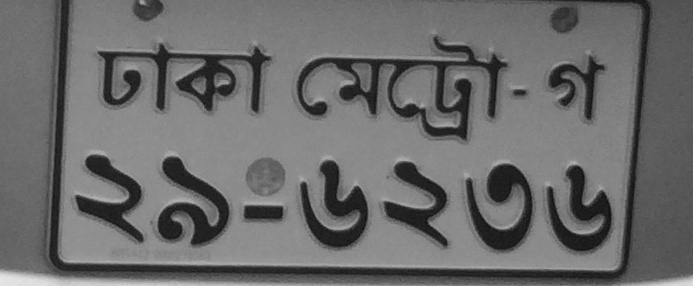
\includegraphics[width=0.9\linewidth]{./img/experiment/stage.9/00-angle2}
    \caption{Original}
\end{subfigure}
\begin{subfigure}{0.33\textwidth}
    \centering
    
\includegraphics[width=0.9\linewidth]{./img/experiment/stage.10/00-angle2}
    \caption{Threshold applied}
\end{subfigure}
\begin{subfigure}{0.33\textwidth}
    \centering
    
\includegraphics[width=0.9\linewidth]{./img/experiment/stage.11/00-angle2}
    \caption{Canny edges}
\end{subfigure}
\caption{Canny edges of an angled plate}
\label{fig:CannyResult2}
\end{figure}

\begin{figure}
\begin{subfigure}{0.33\textwidth}
    \centering
    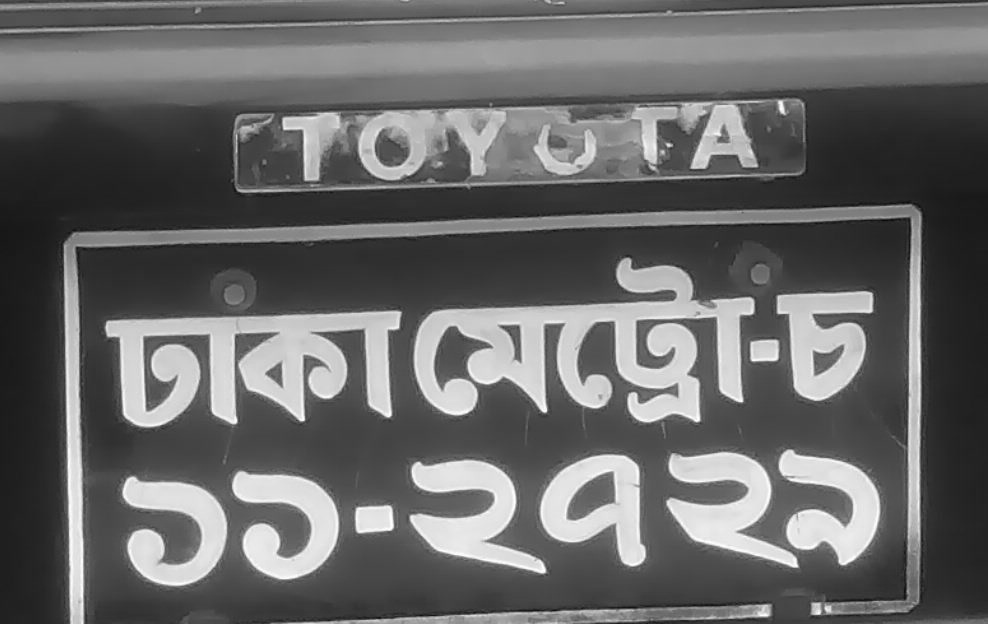
\includegraphics[width=0.9\linewidth]{./img/experiment/stage.9/02-private}
    \caption{Original}
\end{subfigure}
\begin{subfigure}{0.33\textwidth}
    \centering
    
\includegraphics[width=0.9\linewidth]{./img/experiment/stage.10/02-private}
    \caption{Threshold applied}
\end{subfigure}
\begin{subfigure}{0.33\textwidth}
    \centering
    
\includegraphics[width=0.9\linewidth]{./img/experiment/stage.11/02-private}
    \caption{Canny edges}
\end{subfigure}
\caption{Canny edges of a private plate}
\label{fig:CannyResult3}
\end{figure}


\begin{figure}
\begin{subfigure}{0.33\textwidth}
    \centering
    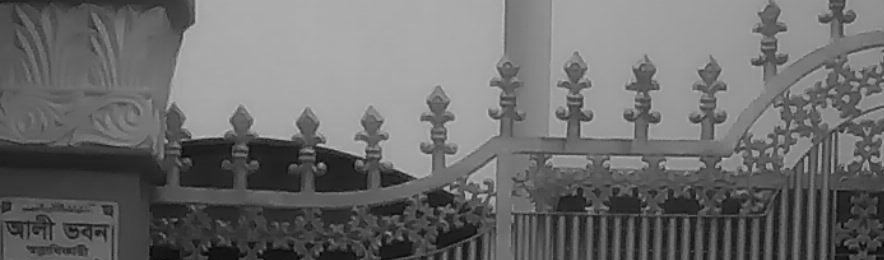
\includegraphics[width=0.9\linewidth]{./img/experiment/stage.9/02-small}
    \caption{Original}
\end{subfigure}
\begin{subfigure}{0.33\textwidth}
    \centering
    
\includegraphics[width=0.9\linewidth]{./img/experiment/stage.10/02-small}
    \caption{Threshold applied}
\end{subfigure}
\begin{subfigure}{0.33\textwidth}
    \centering
    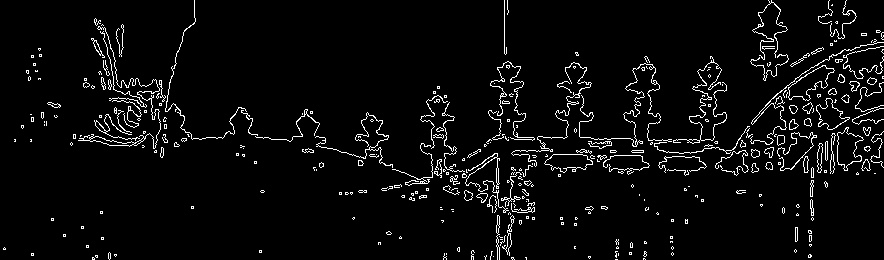
\includegraphics[width=0.9\linewidth]{./img/experiment/stage.11/02-small}
    \caption{Canny edges}
\end{subfigure}
\caption{Canny edges of a bad estimation}
\label{fig:CannyResult4}
\end{figure}

